\begin{figure}[H]
    \centering
    
    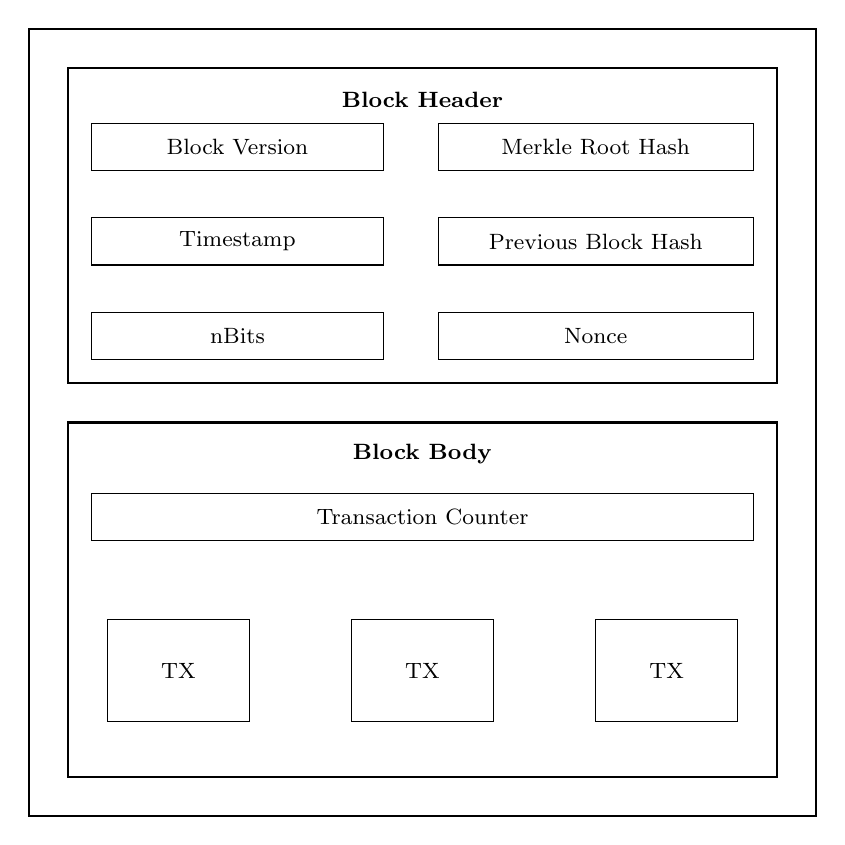
\begin{tikzpicture}[
        node distance=2cm,
        every node/.style={
            font=\footnotesize
        }
    ]
        % Block 1
        \begin{scope}[xshift=0cm]
            \draw[thick] (0,0) rectangle (10,10);
            
            % HEADER 
            \draw[thick] (0.5,5.5) rectangle (9.5,9.5);
            
            \node at (5,9.1) {\textbf{Block Header}};
            
            \draw (0.8,8.2) rectangle (4.5,8.8);
            \node at (2.65,8.5) {Block Version};
            
            \draw (5.2,8.2) rectangle (9.2,8.8);
            \node at (7.2,8.5) {Merkle Root Hash};
            
            \draw (0.8,7.0) rectangle (4.5,7.6);
            \node at (2.65,7.3) {Timestamp};
            
            \draw (5.2,7.0) rectangle (9.2,7.6);
            \node at (7.2,7.3) {Previous Block Hash};
            
            \draw (0.8,5.8) rectangle (4.5,6.4);
            \node at (2.65,6.1) {nBits};
            
            \draw (5.2,5.8) rectangle (9.2,6.4);
            \node at (7.2,6.1) {Nonce};
            
            % BODY 
            \draw[thick] (0.5,0.5) rectangle (9.5,5);
            
            \node at (5,4.6) {\textbf{Block Body}};
            
            \draw (0.8,3.5) rectangle (9.2,4.1);
            \node at (5,3.8) {Transaction Counter};
            
            \draw (1,1.2) rectangle (2.8,2.5);
            \node at (1.9,1.85) {TX};
            
            \draw (4.1,1.2) rectangle (5.9,2.5);
            \node at (5,1.85) {TX};
            
            \draw (7.2,1.2) rectangle (9,2.5);
            \node at (8.1,1.85) {TX};
        \end{scope}
    \end{tikzpicture}
    
    \caption{A block properties}
    
    \label{fig:block_properties}
\end{figure}